\documentclass[]{article}
\usepackage{amsmath}
\usepackage{amssymb}
\usepackage{graphicx}

\title{Physics 229}
% \author[1]{Andrew MacRae}
% \affil[1]{D of P and A, U of V}
\begin{document}
\section{Amplifiers}
\subsection{Active vs. Passive Circuits}
We now move into the regime of so-called \textit{active electronics}. Everything studied so far -- resistors and capacitors, to voltage dividers and filters, to diode rectifiers has fallen under the realm of passive electronics. Active electronic devices, in addition to standard inputs and outputs, require additional power supplies in order to function. There are great benefits to this, as we shall see: active components can output more power than at their input, and can eliminate annoying effects such as voltage loading due to input and output impedance. The first active device we'll study is the amplifier.
\subsection{The Ideal Voltage Amplifier}
The idea of the basic amplifier is simple: take the input $x_\text{in}$ and produce an output which is some number $G$ times the output.
\begin{equation}
\label{eq:simple_amp}
x_\text{out} = Gx_\text{in}
\end{equation}

\noindent ... where $G$ is known as the gain.

There is the question of what input $x_\text{in}$ is being amplified. In our course, normally $x_\text{in}$ will be a voltage and so we will have a voltage amplifier. In this case the gain is often expressed in decibals as:

\begin{equation}
\label{eq:voltage_amp_dB}
G_\text{dB} = 20\log\frac{v_\text{out}}{v_\text{in}} 
\end{equation}

We will occasionally deal with power amplifiers whose input and output is a power. For these amplifiers, the gain is also in dB but with a 10 instead of a 20 multiplier\footnote{Recall that for a fixed load resistance, $P = v^2/R \propto v^2$. Thus $10\log\left[P_\text{out}/P\text{in}\right] = 10\log\left[\left(v_\text{out}/v\text{in}\right)^2\right] = 20\log\left[v_\text{out}/v_\text{in}\right]$, thus yielding consistant definitions of gain}:

\begin{equation}
\label{eq:power_amp_dB}
G_\text{dB} = 10\log\frac{P_\text{out}}{P_\text{in}} 
\end{equation}

\noindent For now though, we will restrict outselves to voltage amplifiers. Diagrammed in figure \ref{fig:simple_amp}. The output is descibed by equation \ref{eq:simple_amp}.

\begin{figure}[h]
\caption{The simplest of amplifiers: the output is the input multiplied by a constant gain $G$.}
\label{fig:simple_amp}
\begin{center}
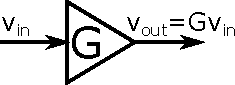
\includegraphics{Images/SimpleAmplifier.pdf}
\end{center}
\end{figure}

\subsection{Reality Check: Amplifiers in Real Life}
There are several limitations to the ideal amplifier that come into effect in practice. For example the amplifier will have to draw at least a small current from the source in order to operate. As we've learned, this is equivalent to a finite \textit{input impedance} $R_\text{in}$. The amplifier will also have a limit to how much current it can output due to its internal resistances. This leads to a finite \textit{output impedance} $R_{out}$. There are also limits to how fast the amplifier can respond to a changing input signal. This leads to a finite \textit{gain bandwidth}, or in general, a frequency dependant gain $G(\omega)$. We will examine each of these effects presently.

\subsubsection{Effects of Finite Input Impedance}
\label{sec:AMP_effect_input}
We can model the non-ideal amplifier as an ideal amplifier inside a black box, precisely as we did with ideal vs real voltage sources. Inside the black-box, the input impedance is models as an internal resistance $R_\text{in}$ to ground placed before the ideal amplifier. This forms a voltage divider with the input impedance from the rest of the circuit so that there is some voltage drop. The ideal amplifier thus sees a different voltage than $v_\text{in}$, which we denote $v^\prime_\text{in}$. The output of the real amplifier is thus less than we would expect: $v_\text{out} = Gv^\prime_\text{in} < Gv_\text{in}$
\begin{figure}[h]
\caption{We model the finite input impedance of the amplifier as a internal resistor $R_\text{in}$ to ground before an ideal amplifier all in a black box.}
\label{fig:real_amp_int}
\begin{center}
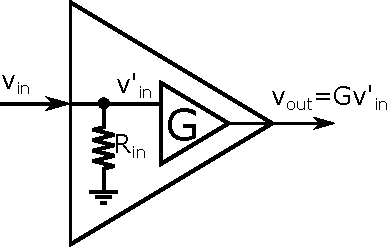
\includegraphics{Images/RealAmplifier_int.pdf}
\end{center}
\end{figure}

The true output, given the input impedance can be calculated given the output impedance of whatever follows. For example, with a $100$~$\Omega$ input impedance amplifier with $G = 10$, 

\subsubsection{Effects of Finite Output Impedance}
The operation of our ideal amplifier can be seen as a two part process: first it senses the voltage at its input (with the effect of finite input impedance causing some loading error), and second, it acts as a new voltage source, producing a voltage $v_\text{out} Gc_\text{in}$. As with any \textit{real} source, it will be equivalent to an ideal source, in series with an output impedance $R_\text{out}$. This finite output impedance leads to a maximum short-circuit current of $v_\text{out}/R_\text{out}$ and will lead to all of the loading issues discussed in chapter XXX. Figure \ref{fig:real_amp_int_out} shows our improved model of how a real amplifier behaves.
\begin{figure}[h]
\caption{A better model of a real amplifier has an input resistance to ground in parallel with the inpput and an output resistance in series with its output.}
\label{fig:real_amp_int_out}
\begin{center}
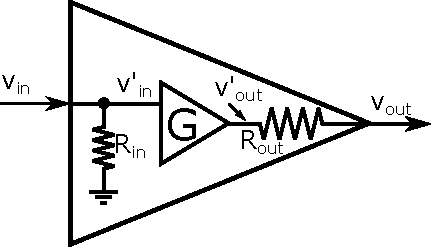
\includegraphics{Images/RealAmplifier_int_out.pdf}
\end{center}
\end{figure}

\noindent\textbf{Design Example:} Consider a real amplifier with $R_\text{in} = 10$~k$\Omega$, $R_\text{F} = 100~\Omega$, and G = 25. We use it to amplify a 10~mV signal from a photodetector having $R_\text{out,PD} = 1250~\Omega$ and send it to a (lousy) voltmeter with $R_\text{in,LVM}$ = 500~$\Omega$ (see figure \ref{fig:prob_amp}). What is the voltage measured (a) assuming an ideal $G = 25$ amplifier, and (b) with our real amplifier?\\\\\noindent Answer: For part (a) the answer is simply $v_\text{meas} = 25\times10~$mV = 250~mV. For our real amplifier, we must consider the input and output stage. The input now forms a voltage divider with $R_\text{in}$ (figure \ref{fig:prob_amp}b so that the inner ideal amplifier sees:
$$
v_\text{in}^\prime=\frac{R_\text{in}}{R_\text{out,PD} + R_\text{in}} = \frac{10~\text{k}\Omega}{11.25~\text{k}\Omega}\times10~\text{mV} \approx 8.9~\text{mV}
$$
In our model, this is then amplified by the ideal internal amplifier producing
$$
v_\text{out}^\prime = 8.9~\text{mV}\times 25 \approx 222~\text{mV}
$$
Finally, this is then sent to our lousy voltmeter, through its internal output resistance, forming another voltage divider (figure \ref{fig:prob_amp}c) to yeild the final voltage:
$$
v_\text{out} = \frac{R_\text{in,LVM}}{R_\text{out} + R_\text{in,LVM}}v_\text{out}^\prime = \frac{500~\Omega}{600~\Omega}\times 222~\text{mV}\approx 185~\text{mV}
$$

\begin{figure}[ht]
\caption{Example Problem.}
\label{fig:prob_amp}
\begin{center}
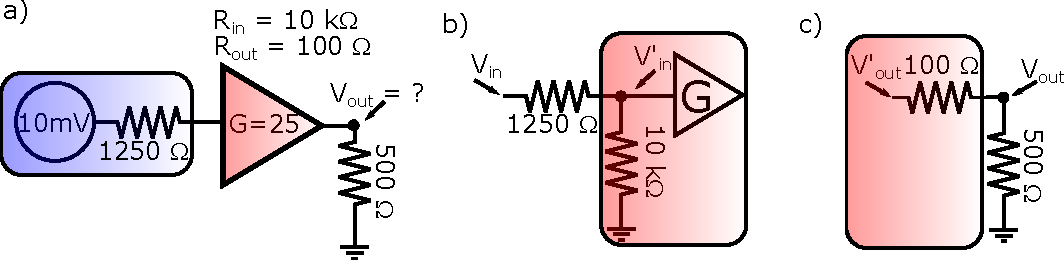
\includegraphics[width=\textwidth]{Images/amp_example.pdf}
\end{center}
\end{figure}

We thus see that the effect of finite input and output impedance is to lessen the effective gain of the real amplifier. Even if we used an ideal voltmeter with infinite input impedance, we'd still see 222~mV $<$ 250~mV. Equivalently, we could try to build an amplifier with $R_\text{out} \rightarrow 0~\Omega$ and again we'd see 222~mV, regardless of the impedance of the voltmeter. To get the full 250~mV however, we'd need to also have $R_\text{in} \rightarrow \infty$, so that $v_\text{in}^\prime = v_\text{in} = 25$~mV. 

From this we can infer the ideal characteristrics of a real amplifier: we want the input impedance as high as possible while having output impedance as low as possible. This can be accomplished using solid state transistors, discussed later in the course. 

\subsection{Effects of Noise: Noise Factor and SNR}
The ideal amplifier will amplify the voltage present at it's input, regardless of whether we consider that voltage to be useful signal or to be noise. This can lead to fundamental issues in isolating very weak signals since eventually, we will just be scaling up Johnson, Shot, or technical noise. 

For example, if you have a 10~nV signal atop 25~nV of Johnson noise, you can send your signal to a 120~dB amplifier to get 100~mV of signal, but it will still be lost in the Johnson noise, which is now at 250~mV.  We amplified the signal level, but have not improved the signal level as compared to the signal. This ratio of signal vs noise has, in a spark of linguistic creativity, been dubbed the ``signal to noise ratio'' or SNR. since the voltage of the noise is usually stochastic \footnote{ A high-brow term, effectively meaning ``random''}, usually the signal to noise ratio is usually specified in terms of power, rather than voltage\footnote{ ...wait, what $R$ should we use here? Well power is energy per unit time and that energy has to be delivered to something. That something is the load resistance, so that a given voltage noise will deliver more power to a 1$00~\Omega$ than a $100~\text{k}\Omega$ resistor} (ie. $v_{RMS}^2/R)$

\begin{equation}
\label{eq:def_snr}
\text{SNR} \equiv \frac{P_\text{sig}}{P_\text{noise}} = 10\log_{10}\left[\frac{P_\text{sig}}{P_\text{noise}}\right] \text{dB}
\end{equation}

So an amplifier on its own will not help you discern signals dominated by noise and the SNR must be improved though separate means. If your signal exits within a given range of frequencies but your noise exists at all frequencies, a filter can be applied to the input of the amplifier to greatly improve the SNR. If the  signal and noise coexist at the same range of frequencies, you have to be more clever. For example, a common source of noise is thermal motion of electrons through a load resistance. To improve the SNR, circuits are often cooled to -40 $^\circ$C or even as low as several Kelvin, when extremely faint signals are being detected.

To make matters worse, the amplifier often adds its own noise to the system - that is the SNR of the output is typically even higher than that of the input! This is quantified by the so-called noise figure:

\begin{equation}
\label{eq:def_noise_figure}
\text{NF} \equiv \frac{\text{SNR}_\text{out}}{\text{SNR}_\text{in}} = 10\log_{10}\left[\frac{\text{SNR}_\text{out}}{\text{SNR}_\text{in}}\right]
\end{equation}

\noindent Good amplifiers will have NF $2$~dB or less.

\subsubsection{Effects of Finite Frequency Response}
Since every circuit element has some finite capacitance and inductance, we can replace the internal input and output resistances with an input impedance $Z_\text{in}$ and output impedance $Z_\text{out}$. The net effect of this is to produce a frequency dependant gain $G(\omega)$. This can be modelled as internal frequency filter that is applied to the input or output. This bug can be rebranded as a feature as an amplifier may actually filter out high frequency noise present in the signal, as discussed in the previous section.

\subsection{Differential Amplifiers}
Often in physics, it is a small deviation from a fixed value that is of interest rather than the absolute value itself. For example, a beam of light may pick up a small oscillation in intensity as compared to a reference beam when passed through a sample. In this case, a \textit{differential amplifier} may be used. As diagrammed in figure XXX, a differential amplier has two inputs and a single output corresponding to the difference between the signals. This is operation can be seen as first inverting one input and then adding it to the other. The input which is inverted $V_-$ is fitting called the ``inverting input'', while the normal input is verbosely titled the ``non-inverting input'', $V_+$. The multiplication factor is known as the ``differential gain'' $G_\text{diff}$ and is defined through the relation
\begin{equation}
\label{eq:def_diff_amp}
v_\text{out} = G_\text{diff}\left(v_+-v_-\right).
\end{equation}

\textit{Example:} A differential amplifier with $G_\text{diff} = 40$~dB has, at its inputs: $v_+ = 3.7$~mV and $v_- = 4.2$~mV. What is the output voltage?\\\\
\textit{Solution:} The gain of 40~dB implies that $20\log_{10}\frac{v_\text{out}}{v_+-v_-} = 40$, so that $v_\text{out} = 100\left(v_+-v_-\right)$. Since, $\left(v_+-v_-\right) = \left(3.7-4.2\right)~\text{mV} = -0.5~\text{mV}$, we will find $v_\text{out} = -500~$mV.
\subsubsection{Common Mode Gain}
From equation \ref{eq:def_diff_amp}, we expect that if $v_+ = v_-$, we will have $v_\text{out} = 0$ regardless of the value of $v_+$ and $v_-$. In practice however, this is not the case. This can be due, for example, to differences in the input impedances of the individual inputs so that internally, $v_-^\prime \neq v_+^\prime$ even though $v_- = v_+$ (see the previous section \ref{sec:AMP_effect_input}). To quantify this, we define the \textit{common-mode voltage} as the average of the inverting vs. non-inverting input voltages:
\begin{equation}
\label{eq:common_mode_voltage}
v_\text{com} \equiv \frac{v_+-v_-}{2}
\end{equation}

The amount of signal that gets through defines the \textit{common-mode gain}
\begin{equation}
\label{eq:common_mode_gain}
v_\text{out} = G_\text{com}\frac{v_++v_-}{2}
\end{equation}
An ideal differntial amplifier would have $G_\text{com} = 0$ or $-\infty$~dB. The true output of the \textit{real} differential amplifier is thus:
\begin{equation}
\label{eq:real_diff_amp}
v_\text{out} = G_\text{diff}\left(v_+-v_-\right) + G_\text{com}\frac{v_++v_-}{2}.
\end{equation}

\subsubsection{Common Mode Rejection Ratio}
The ``goodness'' of a differential amplifier is how much it behaves like one! Mathematically we can quantify this by saying that for a good differential amp, $G_\text{com} \ll G_\text{diff}$. THis is represented by the so-called ``common-mode rejection ratio'' or CMRR. The CMRR is usually stated in decibels and is given by:
\begin{equation}
\label{eq:def_CMRR}
\text{CMRR} \equiv 20\log_{10}\left[\frac{G_\text{diff}}{G_\text{com}}\right]
\end{equation}
 
 Decent differential amplifiers have CMRR$^\text{s}$ of at least 70~dB but some applications require 120~dB or higher.
%\subsection{Special Purpose Amplifiers}Power amplifiers, Audio Amplifiers, Instrumentation Amplifiers, oh my! Also Lock-In Amplifiers!
\end{document}